% questions.tex —— 2016 年·浙江卷·理科 · 题目内容片段（无答案）
% 由 tools/generate_projects.py 依来源总账自 2016/2016_数学真题_浙江理_试题.md 生成，勿手改（改源 MD 后重跑）


\gkpart{数学}

\begin{gktip}
\textbf{来源说明}：本题面依据固定源 PDF 两页 A3 页面逐题核对，原卷印刷页码 1027–1028。固定源不附答案、不印分值；本文件仅为题面规范源。源内中文标点一律为半角，本文件按项目约定统一为全角；源内异常一律照录并在 \texttt{.work} 版式文件中逐条登记（第 2 题三处平行记号「$\parallel$」与第 20 题两条大绝对值竖线在源文本层缺失、系矢量绘制，已照源补出；第 3 题花括号为私用区分片；第 19 题源内「离心率」因栏边断词分两行，照录连排）。
\end{gktip}

\gkpart{一、选择题}

\begin{question}
\gkti{1}已知集合 \(P=\{x\in\mathbf{R}\mid 1\leqslant x\leqslant 3\}\)，\(Q=\{x\in\mathbf{R}\mid x^{2}\geqslant 4\}\)，则 \(P\cup(\complement_{\mathbf{R}}Q)=\)（　）

\begin{gkopts}(1)
\task （A）\([2,3]\)
\task （B）\((-2,3]\)
\task （C）\([1,2)\)
\task （D）\((-\infty,-2]\cup[1,+\infty)\)
\end{gkopts}

\end{question}
\begin{question}
\gkti{2}已知互相垂直的平面 \(\alpha\)，\(\beta\) 交于直线 \(l\)，若直线 \(m\)，\(n\) 满足 \(m\parallel\alpha\)，\(n\perp\beta\)，则（　）

\begin{gkopts}(2)
\task （A）\(m\parallel l\)
\task （B）\(m\parallel n\)
\task （C）\(n\perp l\)
\task （D）\(m\perp n\)
\end{gkopts}

\end{question}
\begin{question}
\gkti{3}在平面上，过点 \(P\) 作直线 \(l\) 的垂线所得的垂足称为点 \(P\) 在直线 \(l\) 上的投影。由区域 \(\begin{cases} x-2\leqslant 0, \\ x+y\geqslant 0, \\ x-3y+4\geqslant 0 \end{cases}\) 中的点在直线 \(x+y-2=0\) 上的投影构成的线段记为 \(AB\)，则 \(|AB|=\)（　）

\begin{gkopts}(2)
\task （A）\(2\sqrt{2}\)
\task （B）4
\task （C）\(3\sqrt{2}\)
\task （D）6
\end{gkopts}

\end{question}
\begin{question}
\gkti{4}命题“\(\forall x\in\mathbf{R}\)，\(\exists n\in\mathbf{N}^{*}\)，使得 \(n\geqslant x^{2}\)”的否定形式是（　）

\begin{gkopts}(1)
\task （A）\(\forall x\in\mathbf{R}\)，\(\exists n\in\mathbf{N}^{*}\)，使得 \(n<x^{2}\)
\task （B）\(\forall x\in\mathbf{R}\)，\(\forall n\in\mathbf{N}^{*}\)，使得 \(n<x^{2}\)
\task （C）\(\exists x\in\mathbf{R}\)，\(\exists n\in\mathbf{N}^{*}\)，使得 \(n<x^{2}\)
\task （D）\(\exists x\in\mathbf{R}\)，\(\forall n\in\mathbf{N}^{*}\)，使得 \(n<x^{2}\)
\end{gkopts}

\end{question}
\begin{question}
\gkti{5}设函数 \(f(x)=\sin^{2}x+b\sin x+c\)，则 \(f(x)\) 的最小正周期（　）

\begin{gkopts}(2)
\task （A）与 \(b\) 有关，且与 \(c\) 有关
\task （B）与 \(b\) 有关，但与 \(c\) 无关
\task （C）与 \(b\) 无关，且与 \(c\) 无关
\task （D）与 \(b\) 无关，但与 \(c\) 有关
\end{gkopts}

\Needspace{0.4\textheight}
\end{question}
\begin{question}
\gkti{6}如图，点列 \(\{A_{n}\}\)，\(\{B_{n}\}\) 分别在某锐角的两边上，且 \(|A_{n}A_{n+1}|=|A_{n+1}A_{n+2}|\)，\(A_{n}\neq A_{n+2}\)，\(n\in\mathbf{N}^{*}\)，\(|B_{n}B_{n+1}|=|B_{n+1}B_{n+2}|\)，\(B_{n}\neq B_{n+2}\)，\(n\in\mathbf{N}^{*}\)（\(P\neq Q\) 表示点 \(P\) 与 \(Q\) 不重合）。若 \(d_{n}=|A_{n}B_{n}|\)，\(S_{n}\) 为 \(\triangle A_{n}B_{n}B_{n+1}\) 的面积，则（　）
\nopagebreak[4]
\begin{center}% 第 6 题点列图：按固定源 PDF 矢量路径换算（1 pt → 0.03515 cm）。
% 原点取下边射线的左端（源页 (155.6289, 652.3750) pt），y 向上。
% 两条截断射线（角顶点在图外，源图有意不画）；三个浅灰填充三角形 S1/S2/Sn；
% 点列 A1..A(n+1) 在上射线、B1..B(n+1) 在下水平线（等距 20.22 pt）；17 组文字标签（A 行 6 + S 行 5 + B 行 6，含 4 组省略号）。
% 注：两射线已画端点纵向相距 23.05 pt、横向错开仅 0.40 pt（被同一竖直截断线切齐），
% 判为有意截断（交点外推约 (114.5, 652.4)），照源复刻不补顶点。
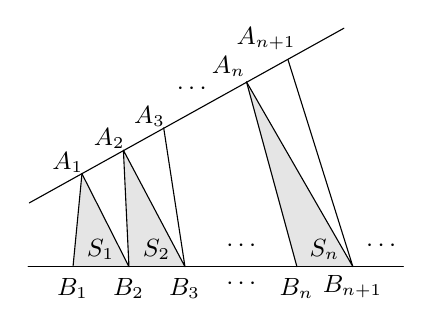
\begin{tikzpicture}[line cap=round,line join=round,font=\small,x=0.03515cm,y=0.03515cm]
% ===== 浅灰填充三角形（fill-opacity 0.1）=====
\fill[black,fill opacity=0.1] (19.41,33.57)--(16.18,0)--(36.39,0)--cycle;
\fill[black,fill opacity=0.1] (34.38,42.06)--(56.62,0)--(36.39,0)--cycle;
\fill[black,fill opacity=0.1] (78.86,66.73)--(97.06,0)--(117.28,0)--cycle;
% ===== 线画 =====
\draw (135.48,0)--(0,0);                 % 下边（水平射线，B 点列所在）
\draw (114.04,86.14)--(0.40,23.05);      % 上边（斜射线，A 点列所在）
\draw (19.41,33.57)--(16.18,0);          % A1B1
\draw (19.41,33.57)--(36.39,0)--(34.38,42.06)--(56.62,0)--(48.93,50.15);  % A1→B2→A2→B3→A3
\draw (78.86,66.73)--(97.06,0);          % AnBn
\draw (78.86,66.73)--(117.28,0)--(93.82,74.82);  % An→Bn+1→An+1
% ===== 文字标签（照源字形框中心，显式坐标）=====
\node[anchor=center,inner sep=0] at (14.30,37.75) {\(A_{1}\)};
\node[anchor=center,inner sep=0] at (29.27,46.25) {\(A_{2}\)};
\node[anchor=center,inner sep=0] at (43.83,54.34) {\(A_{3}\)};
\node[anchor=center,inner sep=0] at (59.05,64.27) {\(\cdots\)};
\node[anchor=center,inner sep=0] at (72.36,72.33) {\(A_{n}\)};
\node[anchor=center,inner sep=0] at (85.92,82.25) {\(A_{n+1}\)};
\node[anchor=center,inner sep=0] at (26.11,6.21) {\(S_{1}\)};
\node[anchor=center,inner sep=0] at (46.34,6.21) {\(S_{2}\)};
\node[anchor=center,inner sep=0] at (76.93,7.65) {\(\cdots\)};
\node[anchor=center,inner sep=0] at (107.02,6.21) {\(S_{n}\)};
\node[anchor=center,inner sep=0] at (127.50,7.65) {\(\cdots\)};
\node[anchor=center,inner sep=0] at (15.99,-7.74) {\(B_{1}\)};
\node[anchor=center,inner sep=0] at (36.22,-7.74) {\(B_{2}\)};
\node[anchor=center,inner sep=0] at (56.45,-7.74) {\(B_{3}\)};
\node[anchor=center,inner sep=0] at (76.93,-6.30) {\(\cdots\)};
\node[anchor=center,inner sep=0] at (96.91,-7.74) {\(B_{n}\)};
\node[anchor=center,inner sep=0] at (117.13,-7.32) {\(B_{n+1}\)};
\end{tikzpicture}
\end{center}
\nopagebreak[4]
\begin{gkopts}(2)
\task （A）\(\{S_{n}\}\) 是等差数列
\task （B）\(\{S_{n}^{2}\}\) 是等差数列
\task （C）\(\{d_{n}\}\) 是等差数列
\task （D）\(\{d_{n}^{2}\}\) 是等差数列
\end{gkopts}

\end{question}
\begin{question}
\gkti{7}已知椭圆 \(C_{1}:\dfrac{x^{2}}{m^{2}}+y^{2}=1\)（\(m>1\)）与双曲线 \(C_{2}:\dfrac{x^{2}}{n^{2}}-y^{2}=1\)（\(n>0\)）的焦点重合，\(e_{1}\)，\(e_{2}\) 分别为 \(C_{1}\)，\(C_{2}\) 的离心率，则（　）

\begin{gkopts}(1)
\task （A）\(m>n\) 且 \(e_{1}e_{2}>1\)
\task （B）\(m>n\) 且 \(e_{1}e_{2}<1\)
\task （C）\(m<n\) 且 \(e_{1}e_{2}>1\)
\task （D）\(m<n\) 且 \(e_{1}e_{2}<1\)
\end{gkopts}

\end{question}
\begin{question}
\gkti{8}已知实数 \(a\)，\(b\)，\(c\)。（　）

（A）若 \(|a^{2}+b+c|+|a+b^{2}+c|\leqslant 1\)，则 \(a^{2}+b^{2}+c^{2}<100\)　（B）若 \(|a^{2}+b+c|+|a^{2}+b-c|\leqslant 1\)，则 \(a^{2}+b^{2}+c^{2}<100\)

（C）若 \(|a+b+c^{2}|+|a+b-c^{2}|\leqslant 1\)，则 \(a^{2}+b^{2}+c^{2}<100\)　（D）若 \(|a^{2}+b+c|+|a+b^{2}-c|\leqslant 1\)，则 \(a^{2}+b^{2}+c^{2}<100\)

\end{question}
\gkpart{二、填空题}

\begin{question}
\gkti{9}若抛物线 \(y^{2}=4x\) 上的点 \(M\) 到焦点的距离为 10，则 \(M\) 到 \(y\) 轴的距离是 \(\underline{\qquad}\)。

\end{question}
\begin{question}
\gkti{10}已知 \(2\cos^{2}x+\sin 2x=A\sin(\omega x+\varphi)+b\)（\(A>0\)），则 \(A=\) \(\underline{\qquad}\)，\(b=\) \(\underline{\qquad}\)。

\Needspace{0.4\textheight}
\end{question}
\begin{question}
\gkti{11}某几何体的三视图如图所示（单位：cm），则该几何体的表面积是 \(\underline{\qquad}\) cm²，体积是 \(\underline{\qquad}\) cm³。
\nopagebreak[4]
\begin{center}% 第 11 题三视图：按固定源 PDF 矢量路径换算（1 pt → 0.03515 cm）。
% 原点取正视图左下角（源页 (524.5664, 375.2969) pt），y 向上。网格 28.1953 pt = 2 cm。
% 正视图：2×2 格、左上格缺（中竖贯通、中横仅左半；按源矢量路径复核）；侧视图：2×2 格、右上格缺（中横贯通、
% 中竖下半为虚线——源内线型如此，按源照录）；俯视图：左列满深、右列只余上半。
% 尺寸标注：横向 4 条 + 竖向 2 条尺寸线（均两段让位给数字），6 条竖直刻度线、3 条水平刻度线，
% 12 个实心箭头（横向一律朝外）；「2」「正视图」「侧视图」「俯视图」共 9 个标签。
\begin{tikzpicture}[line cap=round,line join=round,font=\small,x=0.03515cm,y=0.03515cm]
% ===== 正视图（左格）=====
\draw (0,0)--(56.39,0)--(56.39,56.39)--(28.20,56.39)--(28.20,28.20)--(0,28.20)--cycle;
\draw (28.20,0)--(28.20,28.20);                 % 中竖下半（实线）
% ===== 侧视图（右格，右移 84.58）=====
\draw (84.58,0)--(140.97,0)--(140.97,28.20)--(112.78,28.20)--(112.78,56.39)--(84.58,56.39)--cycle;
\draw (84.58,28.20)--(112.78,28.20);            % 中横左半（实线）
\draw[dash pattern=on 2.99pt off 2.99pt] (112.78,0)--(112.78,28.20);  % 中竖下半（虚线，照源）
% ===== 俯视图 =====
\draw (0,-28.20)--(28.20,-28.20)--(28.20,-84.58)--(0,-84.58)--cycle;   % 左列满深
\draw (28.20,-28.20)--(56.39,-28.20)--(56.39,-56.39)--(28.20,-56.39);  % 右列只余上半（第四边与左列右边重合）
% ===== 尺寸线（横向 4 条 @y=62.03，两段让位）=====
\draw (3.59,62.03)--(24.61,62.03);   \draw (31.78,62.03)--(52.80,62.03);     % 正视图两格
\draw (88.17,62.03)--(109.19,62.03); \draw (116.36,62.03)--(137.39,62.03);  % 侧视图两格
% ===== 尺寸线（竖向 2 条 @x=62.03，两段让位）=====
\draw (62.03,31.78)--(62.03,52.81);  % 上段（高 2）
\draw (62.03,3.59)--(62.03,24.61);   % 下段（高 2）
% ===== 竖直刻度线（6 条，@y 59.21–67.67）=====
\draw (0,59.21)--(0,67.67);        \draw (28.20,59.21)--(28.20,67.67);
\draw (56.39,59.21)--(56.39,67.67); \draw (84.58,59.21)--(84.58,67.67);
\draw (112.78,59.21)--(112.78,67.67); \draw (140.97,59.21)--(140.97,67.67);
% ===== 水平刻度线（3 条，@x 59.21–67.67）=====
\draw (59.21,0)--(67.67,0);
\draw (59.21,28.20)--(67.67,28.20);
\draw (59.21,56.39)--(67.67,56.39);
% ===== 实心箭头（12 个，底 2.98 长 3.98，横向一律朝外）=====
\fill (0,62.03)--(3.98,60.54)--(3.98,63.52)--cycle;         % 正左格：左端←
\fill (28.20,62.03)--(24.22,60.54)--(24.22,63.52)--cycle;   % 正左格：右端→
\fill (28.20,62.03)--(32.18,60.54)--(32.18,63.52)--cycle;   % 正右格：左端←
\fill (56.39,62.03)--(52.41,60.54)--(52.41,63.52)--cycle;   % 正右格：右端→
\fill (84.58,62.03)--(88.56,60.54)--(88.56,63.52)--cycle;   % 侧左格：左端←
\fill (112.78,62.03)--(108.80,60.54)--(108.80,63.52)--cycle;% 侧左格：右端→
\fill (112.78,62.03)--(116.76,60.54)--(116.76,63.52)--cycle;% 侧右格：左端←
\fill (140.97,62.03)--(136.99,60.54)--(136.99,63.52)--cycle;% 侧右格：右端→
\fill (62.03,56.39)--(60.54,52.41)--(63.52,52.41)--cycle;   % 上段：上端↑
\fill (62.03,28.20)--(60.54,32.18)--(63.52,32.18)--cycle;   % 上段：下端↓
\fill (62.03,28.20)--(60.54,24.22)--(63.52,24.22)--cycle;   % 下段：上端↑
\fill (62.03,0)--(60.54,3.99)--(63.52,3.99)--cycle;         % 下段：下端↓
% ===== 标签（照源字形框中心，显式坐标）=====
\node[anchor=center,inner sep=0] at (14.30,66.90) {\(2\)};
\node[anchor=center,inner sep=0] at (42.51,66.90) {\(2\)};
\node[anchor=center,inner sep=0] at (98.92,66.90) {\(2\)};
\node[anchor=center,inner sep=0] at (127.12,66.90) {\(2\)};
\node[anchor=center,inner sep=0] at (67.89,41.51) {\(2\)};
\node[anchor=center,inner sep=0] at (67.89,13.31) {\(2\)};
\node[anchor=center,inner sep=0] at (28.40,-13.54) {正视图};
\node[anchor=center,inner sep=0] at (113.01,-13.54) {侧视图};
\node[anchor=center,inner sep=0] at (28.40,-98.09) {俯视图};
\end{tikzpicture}
\end{center}
\nopagebreak[4]
\end{question}
\begin{question}
\gkti{12}已知 \(a>b>1\)。若 \(\log_{a}b+\log_{b}a=\dfrac{5}{2}\)，\(a^{b}=b^{a}\)，则 \(a=\) \(\underline{\qquad}\)，\(b=\) \(\underline{\qquad}\)。

\end{question}
\begin{question}
\gkti{13}设数列 \(\{a_{n}\}\) 的前 \(n\) 项和为 \(S_{n}\)。若 \(S_{2}=4\)，\(a_{n+1}=2S_{n}+1\)，\(n\in\mathbf{N}^{*}\)，则 \(a_{1}=\) \(\underline{\qquad}\)，\(S_{5}=\) \(\underline{\qquad}\)。

\Needspace{0.4\textheight}
\end{question}
\begin{question}
\gkti{14}如图，在 \(\triangle ABC\) 中，\(AB=BC=2\)，\(\angle ABC=120^{\circ}\)。若平面 \(ABC\) 外的点 \(P\) 和线段 \(AC\) 上的点 \(D\)，满足 \(PD=DA\)，\(PB=BA\)，则四面体 \(PBCD\) 的体积的最大值是 \(\underline{\qquad}\)。
\nopagebreak[4]
\begin{center}% 第 14 题四面体图：按固定源 PDF 矢量路径换算（1 pt → 0.03515 cm）。
% 原点取顶点 A（源页 (522.6875, 706.3477) pt），y 向上。
% 顶点：A(0,0)、B(96.36,0)、C(144.54,83.83)、D(41.91,24.09)（在 AC 上，距 A 约 29%）、P(30.84,70.82)。
% 实线 7 段：AB、AD、BD、DP、PB、PC、BC；虚线 1 段：DC（不可见棱）。无箭头。
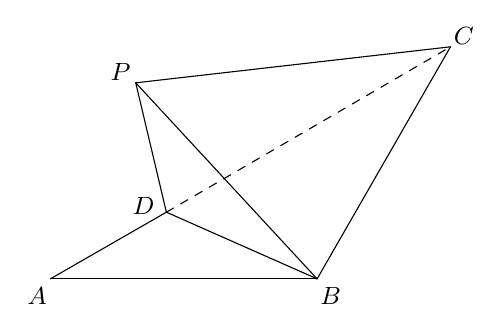
\begin{tikzpicture}[line cap=round,line join=round,font=\small,x=0.03515cm,y=0.03515cm]
% ===== 虚线先画（不可见棱 DC）=====
\draw[dash pattern=on 2.99pt off 2.99pt] (41.91,24.09)--(144.54,83.83);
% ===== 实线 =====
\draw (0,0)--(96.36,0);              % A-B
\draw (0,0)--(41.91,24.09);          % A-D
\draw (96.36,0)--(41.91,24.09);      % B-D
\draw (41.91,24.09)--(30.84,70.82);  % D-P
\draw (30.84,70.82)--(144.54,83.83); % P-C
\draw (30.84,70.82)--(96.36,0);      % P-B
\draw (96.36,0)--(144.54,83.83);     % B-C
% ===== 标注（照源字形框中心，显式坐标）=====
\node[anchor=center,inner sep=0] at (-4.73,-6.06) {\(A\)};
\node[anchor=center,inner sep=0] at (101.26,-6.06) {\(B\)};
\node[anchor=center,inner sep=0] at (149.35,87.67) {\(C\)};
\node[anchor=center,inner sep=0] at (33.70,26.40) {\(D\)};
\node[anchor=center,inner sep=0] at (25.38,74.66) {\(P\)};
\end{tikzpicture}
\end{center}
\nopagebreak[4]
\end{question}
\begin{question}
\gkti{15}已知向量 \(\mathbf{a}\)，\(\mathbf{b}\)，\(|\mathbf{a}|=1\)，\(|\mathbf{b}|=2\)，若对任意单位向量 \(\mathbf{e}\)，均有 \(|\mathbf{a}\cdot\mathbf{e}|+|\mathbf{b}\cdot\mathbf{e}|\leqslant\sqrt{6}\)，则 \(\mathbf{a}\cdot\mathbf{b}\) 的最大值是 \(\underline{\qquad}\)。

\end{question}
\gkpart{三、解答题}

\begin{question}
\gkti{16}在 \(\triangle ABC\) 中，内角 \(A\)，\(B\)，\(C\) 所对的边分别为 \(a\)，\(b\)，\(c\)。已知 \(b+c=2a\cos B\)。

（1） 证明：\(A=2B\)；

（2） 若 \(\triangle ABC\) 的面积 \(S=\dfrac{a^{2}}{4}\)，求角 \(A\) 的大小。

\Needspace{0.4\textheight}
\end{question}
\begin{question}
\gkti{17}如图，在三棱台 \(ABC-DEF\) 中，平面 \(BCFE\perp\) 平面 \(ABC\)，\(\angle ACB=90^{\circ}\)，\(BE=EF=FC=1\)，\(BC=2\)，\(AC=3\)。

（1） 求证：\(BF\perp\) 平面 \(ACFD\)；

（2） 求二面角 \(B-AD-F\) 的平面角的余弦值。
\nopagebreak[4]
\begin{center}% 第 17 题三棱台图：按固定源 PDF 矢量路径换算（1 pt → 0.03515 cm）。
% 原点取顶点 A（源页 (980.7578, 532.9297) pt），y 向上。
% 顶点：A(0,0)、B(109.37,−41.43)、C(152.25,0)、D(65.52,37.58)、E(118.04,21.68)、F(143.57,37.58)。
% 实线 8 段（含题图额外画出的 BF——题干要求证 BF⊥平面 ACFD）；虚线 1 段：AC（被遮挡的底棱）。无箭头。
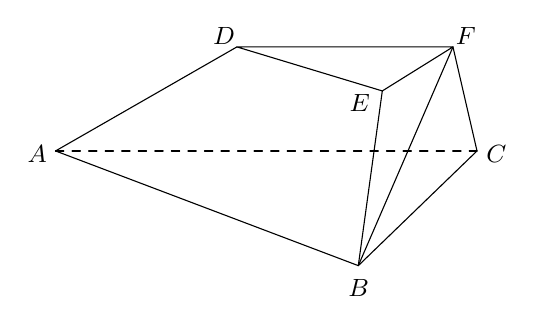
\begin{tikzpicture}[line cap=round,line join=round,font=\small,x=0.03515cm,y=0.03515cm]
% ===== 虚线先画（底棱 AC）=====
\draw[dash pattern=on 2.99pt off 2.99pt] (0,0)--(152.25,0);
% ===== 实线 =====
\draw (109.37,-41.43)--(0,0);        % BA
\draw (109.37,-41.43)--(152.25,0);   % BC
\draw (65.52,37.58)--(0,0);          % DA
\draw (118.04,21.68)--(109.37,-41.43); % EB
\draw (143.57,37.58)--(152.25,0);    % FC
\draw (109.37,-41.43)--(143.57,37.58); % BF（题图额外线段）
\draw (118.04,21.68)--(143.57,37.58)--(65.52,37.58)--cycle; % 上底 DEF（EF、FD、DE）
% ===== 标注（照源字形框中心，显式坐标）=====
\node[anchor=center,inner sep=0] at (-6.60,-1.06) {\(A\)};
\node[anchor=center,inner sep=0] at (109.52,-49.49) {\(B\)};
\node[anchor=center,inner sep=0] at (159.27,-1.06) {\(C\)};
\node[anchor=center,inner sep=0] at (60.84,41.46) {\(D\)};
\node[anchor=center,inner sep=0] at (109.87,17.20) {\(E\)};
\node[anchor=center,inner sep=0] at (148.20,41.46) {\(F\)};
\end{tikzpicture}
\end{center}
\nopagebreak[4]
\end{question}
\begin{question}
\gkti{18}已知 \(a\geqslant 3\)，函数 \(F(x)=\min\{2|x-1|,\ x^{2}-2ax+4a-2\}\)，其中

\nopagebreak[4]
\[
\min\{p,q\}=\begin{cases}
p, & p\leqslant q, \\
q, & p>q.
\end{cases}
\]

（1） 求使得等式 \(F(x)=x^{2}-2ax+4a-2\) 成立的 \(x\) 的取值范围；

（2） ① 求 \(F(x)\) 的最小值 \(m(a)\)；

　　② 求 \(F(x)\) 在区间 \([0,6]\) 上的最大值 \(M(a)\)。

\Needspace{0.4\textheight}
\end{question}
\begin{question}
\gkti{19}如图，设椭圆 \(\dfrac{x^{2}}{a^{2}}+y^{2}=1\)（\(a>1\)）。

（1） 求直线 \(y=kx+1\) 被椭圆截得的线段长（用 \(a\)，\(k\) 表示）；

（2） 若任意以点 \(A(0,1)\) 为圆心的圆与椭圆至多有 3 个公共点，求椭圆离心率的取值范围。
\nopagebreak[4]
\begin{center}% 第 19 题椭圆坐标图：按固定源 PDF 矢量路径换算（1 pt → 0.03515 cm）。
% 原点取椭圆中心 O（源页 (692.9102, 202.0039) pt，即两轴交点），y 向上。
% 椭圆半轴 56.6719/34.0020（轴比 ≈5:3，源为示意画法），线宽 0.8pt（源为其余图元 2 倍）；
% x 轴左 −76.51 右至箭头 76.51、y 轴下 −56.67 上至箭头 59.51（均穿出椭圆，左右不对称照源）；
% 标签 y/A/x/O 四处；A 标于椭圆上顶点（对应题设 A(0,1)）。无实心点、无刻度。
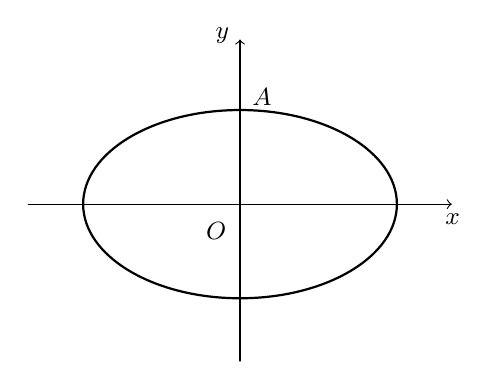
\begin{tikzpicture}[line cap=round,line join=round,font=\small,x=0.03515cm,y=0.03515cm]
% 坐标轴
\draw[->] (-76.51,0)--(76.51,0);
\draw[->] (0,-56.67)--(0,59.51);
% 椭圆（线宽 0.8，与源一致）
\draw[line width=0.8pt] (0,0) ellipse (56.67 and 34.00);
% ===== 标注（照源字形框中心，显式坐标）=====
\node[anchor=center,inner sep=0] at (-6.39,60.94) {\(y\)};
\node[anchor=center,inner sep=0] at (7.91,38.75) {\(A\)};
\node[anchor=center,inner sep=0] at (76.80,-5.57) {\(x\)};
\node[anchor=center,inner sep=0] at (-8.59,-9.66) {\(O\)};
\end{tikzpicture}
\end{center}
\nopagebreak[4]
\end{question}
\begin{question}
\gkti{20}设数列 \(\{a_{n}\}\) 满足 \(\left|a_{n}-\dfrac{a_{n+1}}{2}\right|\leqslant 1\)，\(n\in\mathbf{N}^{*}\)。

（1） 证明：\(|a_{n}|\geqslant 2^{n-1}(|a_{1}|-2)\)，\(n\in\mathbf{N}^{*}\)；

（2） 若 \(|a_{n}|\leqslant\left(\dfrac{3}{2}\right)^{n}\)，\(n\in\mathbf{N}^{*}\)，证明：\(|a_{n}|\leqslant 2\)，\(n\in\mathbf{N}^{*}\)。

\end{question}